
\chapter[Suporte Tecnológico]{Suporte Tecnológico}

Nesta seção, serão apresentadas ferramentas e tecnologias utilizadas para auxiliar o desenvolvimento deste projeto, desde a organização e definição da metodologia de pesquisa, até o desenvolvimento dos projetos pilotos durante o trabalho. Esta seção está dividida em \textit{Engenharia de Software} e \textit{Robótica Educacional}.

\section{Engenharia de software} % (fold)
\label{sec:engenharia_de_software}
	Neste tópico, serão apresentadas ferramentas e tecnologias voltadas ao contexto da Engenharia de Software que são utilizadas durante este trabalho, como, por exemplo, ferramentas para gerência de configuração e versionamento dos artefatos gerados.

	\subsection{GIT} % (fold)
	\label{sub:git}
	
		A ferramenta GIT\footnote{https://git-scm.com/} foi desenvolvida por Linus Torvalds, mesmo criador do Linux, e assim como ele, é \textit{open-source}. Disponibiliza uma eficiente forma de versionamento e gerenciamento de projetos. 
	% subsection git (end)

	\subsection{Github} % (fold)
	\label{sub:github}
		O Github\footnote{https://github.com} é uma ferramenta utilizada para hospedagem remota de projetos GIT. A ferramenta contempla uma \textit{Wiki} para documentação do projeto e sistemas de \textit{Issues} e \textit{Milestones}\footnote{https://guides.github.com/features/issues/} para gerenciamento de atividades.
	% subsection github (end)

	\subsection{Bonita BPMN} % (fold)
	\label{sub:bonita_bpmn}
		Ferramenta para modelagem de processos \textit{BPMN}\footnote{http://www.bpmn.org/}, o Bonita\footnote{http://www.bonitasoft.com/} 7 foi escolhido graças a sua facilidade de utilização e portabilidade para o sistema operacional Linux.
	% subsection bizagi_process_modeler (end)

	\subsection{Linux Mint} % (fold)
	\label{sub:linux_mint}
		O sistema operacional utilizado durante este trabalho é o Linux Mint\footnote{https://www.linuxmint.com/} e o Windows 7 Ultimate\footnote{https://www.microsoft.com/pt-br/software-download/windows7}.
	% subsection linux_mint (end)

	\subsection{LaTeX} % (fold)
	\label{sub:latex}
	
	O LaTeX\footnote{https://www.latex-project.org/} 3.14 é um sistema para criação de documentos utilizando textos \textit{tex}, foi incialmente desenvolvido por Leslie Lamport, na década de 80. O LaTeX oferece diversos comandos avançados para organização de alto nível de documentos, incluindo facilitadores para citações, bibliografias, fórmulas matemáticas, figuras e tabelas.
	% subsection latex (end)

	\subsection{Sublime Text 3} % (fold)
	\label{sub:sublime_text_3}
		O Sublime Text 3\footnote{https://www.sublimetext.com/3} é um editor de texto bastante utilizado por programadores, por possuir apoio para diversas linguagens de programação, incluindo textos em LaTeX.
	% subsection sublime_text_3 (end)

\section{Robótica educacional} % (fold)
\label{sec:robótica_educacional_suporte}

	\subsection{RoboMind 6.0} % (fold)
	\label{sub:robomind}

		É um ambiente de desenvolvimento proposto por Arvid Halma\footnote{http://www.robomind.net/pt/index.html}, da Universidade de Amsterdam, que tem como objetivo facilitar o ensino de programação para estudantes do ensino básico. Utiliza um robô virtual para exercitar os conceitos de inteligência artificial e lógica de programação. A linguagem utilizada é chamada Robo/Roo, e permite implementação da movimentação do robô em um ambiente 2D (duas dimensões). As funções básicas da ferramenta, são \textit{ver}, \textit{andar}, \textit{pegar}, \textit{pintar}, como mosta a Figura \ref{img:funcoesBasicasRoboMind}.

		\begin{figure}[H]
			\centering
			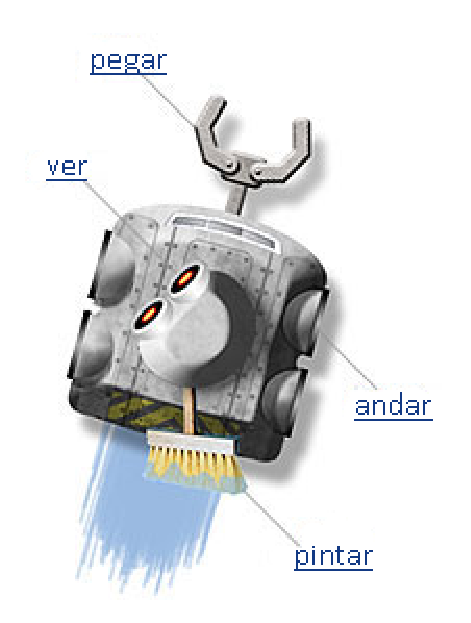
\includegraphics[scale=0.8]{figuras/funcoesBasicasRoboMind.eps}
			\caption[Funções básicas RoboMind]{Funções básicas RoboMind}
			\label{img:funcoesBasicasRoboMind}
		\end{figure}
	
	% subsection robomind (end)

	\subsection{Scratch} % (fold)
	\label{sub:scratch}

		É um ambiente de desenvolvimento criado por Lofelong Kindergarten Group(LLK)\footnote{https://llk.media.mit.edu/projects/}, que é um grupo de pesquisa do MIT. Também tem como objetivo introduzir conceitos de programação a alunos da educação básica. Com a utilização desta ferramenta, é possível desenvolver jogos, animações e histórias interativas, de modo visual.

		A utilização da ferramenta pode ser visualizada na Figura \ref{img:funcoesBasicasScratch}, onde são apresentadas funções básicas no modo visual de desenvolvimento do Scratch.

		\begin{figure}[H]
			\centering
			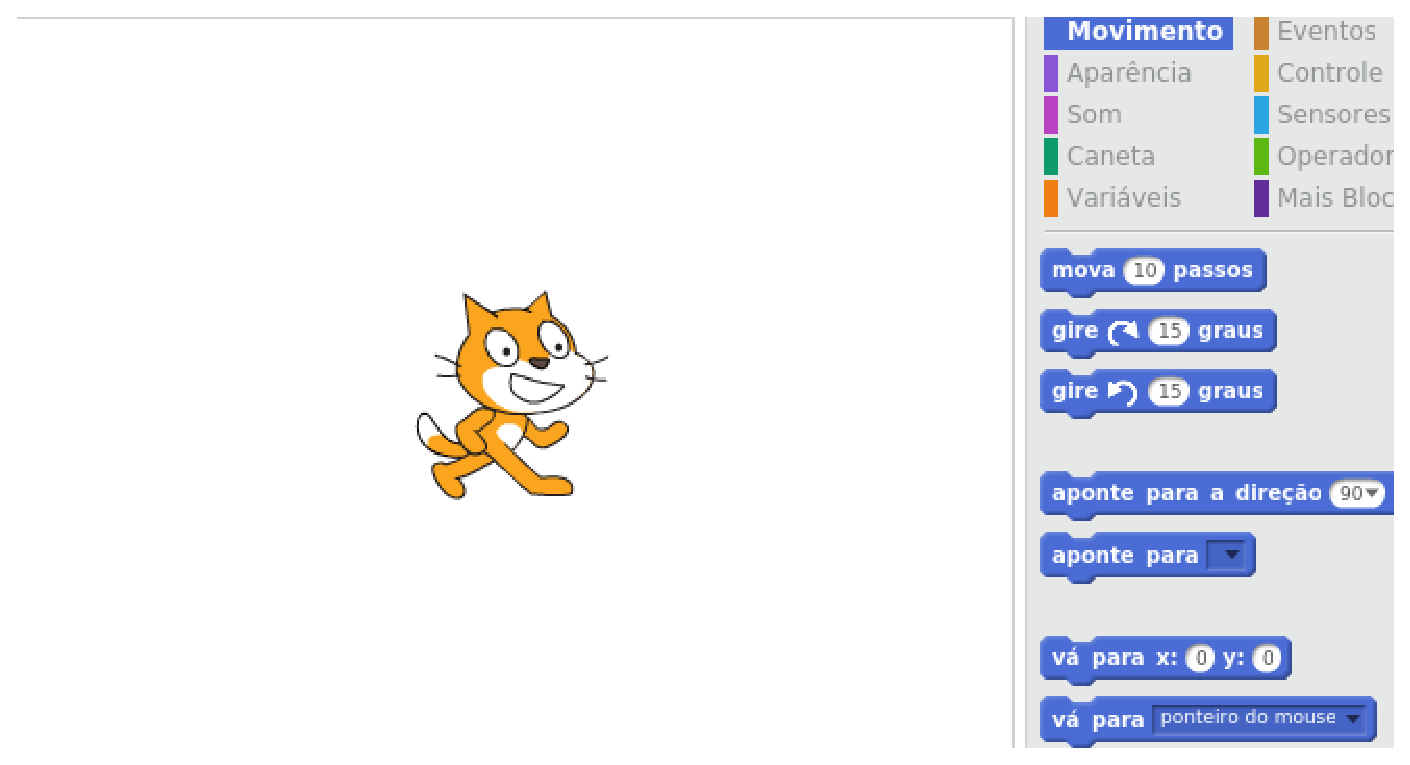
\includegraphics[scale=0.7]{figuras/funcoesBasicasSratch.eps}
			\caption[Funções básicas Scratch]{Funções básicas Scratch}
			\label{img:funcoesBasicasScratch}
		\end{figure}
	% subsection scratch (end)

	\subsection{Linguagem Logo} % (fold)
	\label{sub:linguagem_logo}

		A linguagem Logo\footnote{https://logo.codeplex.com/} também foi desenvolvida em 1967, também pelo MIT. É uma linguagem interpretada, bastante utilizada para o desenvolvimento de inteligência artificial no contexto educacional. Sua utilização também é de forma visual, como apresenta a Figura \ref{img:ambienteLogo}. A caixa de texto visível na Figura \ref{img:ambienteLogo} recebe os comandos para movimentação do robô virtual em um ambiente 2D (duas dimensões).

		\begin{figure}[H]
			\centering
			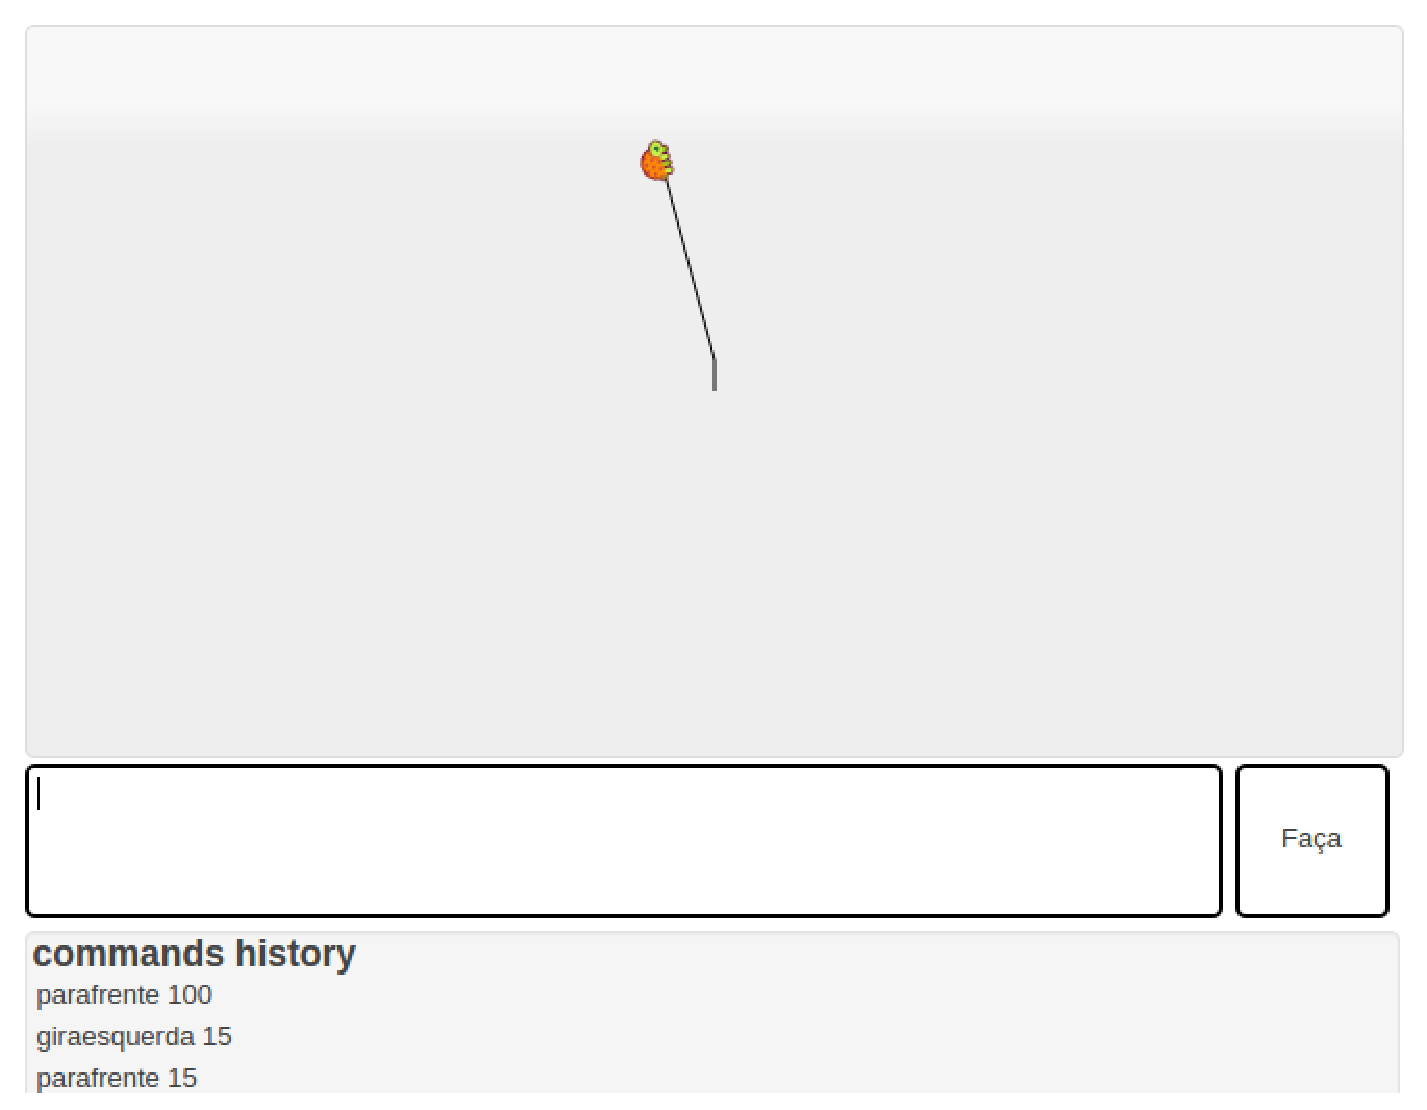
\includegraphics[scale=0.7]{figuras/ambienteLogo.eps}
			\caption[Ambiente de desenvolvimento em Logo]{Ambiente de desenvolvimento em Logo}
			\label{img:ambienteLogo}
		\end{figure}
	% subsection linguagem_logo (end)

	\subsection{Kodu Game Labs} % (fold)
	\label{sub:kodu_game_labs}

		Foi desenvolvido pelo laboratório de pesquisas FUSE (Future Social Experiences)\footnote{https://fuse.microsoft.com/}, que é mantido pela Microsoft. Esta ferramenta possui uma complexidade que não estava presente nas ferramentas apresentadas anteriormente. Seu objetivo é desenvolver jogos em ambiente 3D (três dimensões) no contexto educacional, facilitando o aprendizado de programação orientada a objetos. 

		Os jogos desenvolvidos se baseiam na criação de um mundo completo, com personagens, ações e objetos. Os personagens utilizados podem ser inseridos com funções já pré-definidas, ou o usuário pode programar o personagem da forma que desejar, garantindo a flexibilidade e quantidade de possibilidades da ferramenta.
	
	% subsection kodu_game_labs (end)

	\subsection{Alice 2.0} % (fold)
	\label{sub:alice}
		Assim como o Kodu Game, a ferramenta Alice\footnote{http://www.aliceprogramming.net/} também disponibiliza um ambiente tridimensional para desenvolvimento de animações e jogos interativos. Foi desenvolvida por um grupo de pesquisa liderado por Randy Pausch\footnote{http://www.cs.cmu.edu/~pausch/news/}, da Universidade de Virgínia e Universidade de Carnegie Mellon. Diferentemente do Kodu Game, a ferramenta Alice possui apenas um \textit{Mundo}, onde serão implementadas todas as histórias e relações da animação ou jogo. Após análise da ferramenta, \cite{analiseFerramentaEnsinoComputacao} cita problemas de instabilidade e \textit{bugs}.
	
	% subsection subsection_name (end)

	\subsection{Mindstorms Lego} % (fold)
	\label{sub:mindstorm_lego}

		Os kits de robótica Mindstorms da Lego, diferentemente de todas as ferramentas apresentadas acima, disponibiliza um ambiente real de desenvolvimento. Envolve a implementação de ações dos atuadores presentes em cada robô, onde estas ações serão executadas baseando-se nas informações advindas dos sensores. A especificação desta ferramenta se encontra na seção \ref{sub:kit_mindstorm}.
	
	% subsection subsection_name (end)
% section robótica_educacional (end)
	
\section{Considerações parciais} % (fold)
\label{sec:considerações_parciais}

	Este capítulo buscou apresentar as ferramentas e tecnologias utilizadas para apoiar o desenvolvimento desta pesquisa, desde a realização da revisão sistemática e documentação do projeto, até a análise de abordagens utilizadas na Robótica Educacional. Analisando as ferramentas utilizadas, observa-se que a base tecnológica do trabalho é resumida em componentes gratuitos e, se possível, \textit{open source}.

	A análise das ferramentas citadas se deu com o objetivo de analisar maneiras de se trabalhar o contexto educacional, utilizando ferramentas de apoio e abordagens de ensino. Dentre as ferramentas apresentadas, se encontram ferramentas que apoiam o ensino de diversas áreas de conhecimento, como programação e matemática. Sendo elas ferramentas virtuais ou reais, como é o caso do kit Mindstorm, foco deste trabalho.

% section considerações_parciais (end)

% subsection subsection_name (end)
% section engenharia_de_software (end)